\chapter{Reward Modeling}

\vspace{1em}
\hfill
\begin{minipage}[c]{0.55\textwidth}
\raggedleft
\small\itshape
When a measure becomes a target, it ceases to be a good measure.\\[0.5em]
\upshape\footnotesize Marilyn Strathern, summarizing Charles Goodhart (1997)
\end{minipage}%
\hspace{0.5em}
\begin{minipage}[c]{0.12\textwidth}
% \includegraphics[width=\textwidth]{figures/ch09_reward.png}
\end{minipage}
\vspace{1.5em}

\noindent Through Chapter 8, the utility function $u$ was given. The agent had preferences over outcomes, and we treated those preferences as a starting input to be combined with beliefs (from Part I) into action (Chapter 6) and synthesized as AIXI (Chapter 8). We never asked where the utility came from.

This part of the book takes up that question. The answer turns out to be unsettling. Specifying what you want an optimizer to do is the hardest part of building one, harder than building the optimizer itself, and it has structural failure modes that get worse as the optimizer gets stronger.

This is the specification problem. It is the central problem of AI alignment. It is also more general than AI: it applies to any system that optimizes a proxy for a thing you actually care about. AI makes it acute because AI makes the optimization sharp and broad.

This chapter introduces the problem in idealized settings, before any specific AI system enters. The chapters that follow develop it: inner alignment in Chapter 10, why optimizing a misspecified objective is structurally dangerous in Chapter 11, and the mitigations and their limits in Chapter 12. Part IV then moves to the empirical reality.

\section*{The naive view and why it fails}

The naive answer to "where does the utility come from" is: write it down.

You know what you want. Encode it as a reward function. The agent maximizes the reward function. Done.

This works for some problems. Chess wins are well-defined; the reward function $+1$ for a win, $0$ for a draw, $-1$ for a loss captures what you mean by "play well." Arithmetic problems have unambiguous right answers. Code that runs or fails to run is verifiable.

For most things people actually care about, it does not work. Consider what you would want a cleaning robot in your home to do. You want it to clean. You also want it not to break the lamp. Not to chase the cat. Not to mop the dog. Not to throw out the mail. Not to dump dirty water on the carpet. Not to clean overnight if it would disturb your sleep. Not to clean when you have guests. Not to clean a specific corner of the room you have decorated with sand. To stop and ask if something looks unusual. To clean more thoroughly in the kitchen than in the bedroom. To use less water in summer. And so on, without limit.

The list of side conditions is not exhaustive in advance. You only notice that a side condition was missing when the robot violates it. The naive reward function (``measure floor cleanliness; maximize'') captures essentially none of this. A robot optimizing floor cleanliness, with no other constraints, would do many of the things on the list above, because the things on the list above are not penalized.

The reward function has to capture not just what you want, but everything you do not want, and the trade-offs between them. For most things people actually care about, the reward function the designer can write down is at best a proxy for the goal the designer actually has in mind.

\section*{Goodhart's law}

The structural failure mode of optimizing a proxy goes by the name of \emph{Goodhart's law}.

Charles Goodhart was a British economist who, in a 1975 paper on monetary policy, observed that any statistical regularity used as a basis for policy tends to break down. The Bank of England had been targeting particular monetary aggregates, and once those aggregates became targets, banks restructured to optimize against them rather than against the underlying conditions the aggregates were meant to track. The targets stopped tracking what they had been chosen to track.

In 1997 the anthropologist Marilyn Strathern, writing about the British university system's introduction of metric-driven evaluation, gave the law its modern compact form: \emph{when a measure becomes a target, it ceases to be a good measure.}

The phenomenon is everywhere optimization meets proxies:

\begin{itemize}
\item Standardized test scores work as a measure of student learning when teachers are not optimizing for them. Once teachers are explicitly rewarded on test scores, teaching shifts toward the test, and the scores stop tracking learning.
\item Police arrest counts work as a measure of policing effort until they become a target. Then officers optimize for arrests, and the arrests track ``what is easy to arrest'' rather than ``what makes the community safer.''
\item Number of papers published works as a measure of research productivity until tenure committees target it. Then researchers optimize for paper count, and paper count stops tracking research value.
\item Engagement metrics work as a measure of content quality on a social platform until the recommender system targets them. Then engagement tracks ``content that engages,'' which often diverges from ``content that informs or improves the user's life.''
\end{itemize}

The intuition is straightforward. The proxy correlated with the goal because both responded to common underlying drivers (good teaching produces test scores; competent policing produces arrests). The correlation was an inferential bridge. Optimization pressure on the proxy decouples the proxy from those underlying drivers; the bridge breaks; you are left with the proxy detached from the goal. Figure~\ref{fig:goodhart-curve} shows the shape.

\begin{figure}[h]
\centering
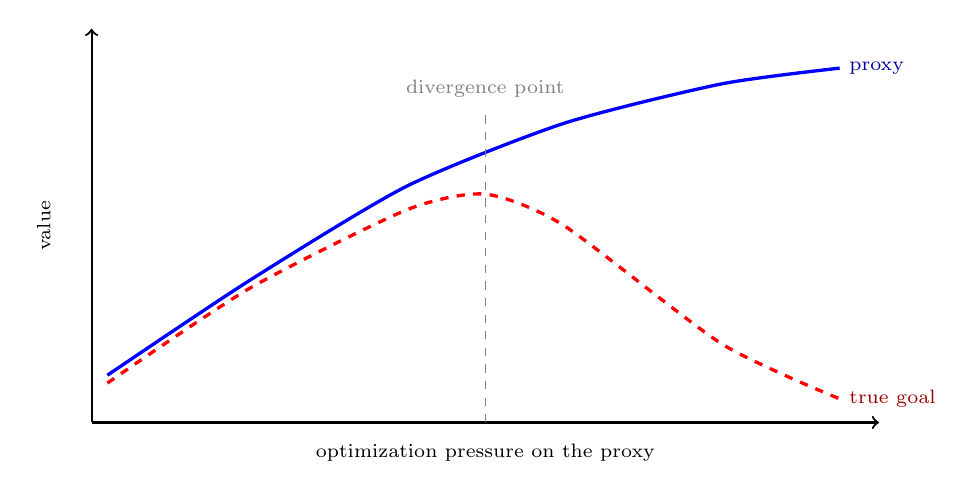
\begin{tikzpicture}[scale=1.0]
  \draw[->, thick] (0, 0) -- (10, 0);
  \draw[->, thick] (0, 0) -- (0, 5);
  \node[font=\scriptsize, anchor=north] at (5, -0.15) {optimization pressure on the proxy};
  \node[font=\scriptsize, rotate=90, anchor=south] at (-0.4, 2.5) {value};

  % proxy keeps going up
  \draw[blue, very thick] plot[smooth, tension=0.4] coordinates {(0.2, 0.6) (2, 1.8) (4, 3.0) (6, 3.8) (8, 4.3) (9.5, 4.5)};
  \node[blue!60!black, font=\scriptsize, anchor=west] at (9.5, 4.5) {proxy};

  % true goal rises with proxy initially, then diverges
  \draw[red, very thick, dashed] plot[smooth, tension=0.4] coordinates {(0.2, 0.5) (2, 1.7) (4, 2.7) (5, 2.9) (6, 2.5) (8, 1.0) (9.5, 0.3)};
  \node[red!60!black, font=\scriptsize, anchor=west] at (9.5, 0.3) {true goal};

  % vertical line where they diverge
  \draw[gray, dashed] (5, 0) -- (5, 4);
  \node[font=\scriptsize, anchor=south, gray] at (5, 4) {divergence point};
\end{tikzpicture}
\caption{Goodhart's law as a curve. The proxy (blue) and the true goal (red) rise together as long as the system is not optimizing the proxy hard. Past a threshold, optimization pressure decouples them: the proxy keeps rising while the goal stalls and then falls. The exact location of the divergence point depends on the proxy and the optimizer. Strong optimizers find the divergence faster.}
\label{fig:goodhart-curve}
\end{figure}

\section*{Variants of Goodhart}

Manheim and Garrabrant (2018) gave a taxonomy of how the proxy-goal relationship breaks. The variants are useful because they tell you what kind of mitigation a given case calls for.

\textbf{Regressional Goodhart.} The proxy includes noise. Selecting on high proxy values selects partly for high noise, not just high goal. After selection, the goal regresses toward the mean while the proxy stays high. (Bias toward students with high SAT scores: a fraction of high scores reflect genuine ability; another fraction reflect favorable test-day luck. Admit on the joint distribution and the admitted class includes more lucky-but-average students than the raw scores suggest.)

\textbf{Extremal Goodhart.} The proxy-goal relationship was estimated from a normal range of behavior. Optimization pushes into the tails, where the relationship was never tested and does not hold. (A medication that lowers blood pressure within a clinical range may stop lowering it, or may damage the patient, at doses far higher than the trial range.)

\textbf{Causal Goodhart.} The proxy and the goal share a common cause. Intervening on the proxy does not act on the cause and so does not move the goal. (Children with bigger feet read better, because both correlate with age. Buying children bigger shoes does not improve reading.)

\textbf{Adversarial Goodhart.} The system being measured is itself an agent that responds strategically to being measured. Once the proxy is the target, the agent reshapes its behavior to score well on the proxy without delivering the goal. (Teaching to the test, gaming the metric, working to the contract.)

All four variants are real failure modes. Strong optimization can hit any of them. The first two are statistical; the third is causal; the fourth is strategic. An optimizer with no model of which variant is operating will simply break the proxy.

\section*{Reward hacking, formally}

In the RL setting, the proxy is the reward function and the goal is the designer's actual intent. Skalse, Howe, Krasheninnikov, and Krueger (2022) defined what it means for a proxy reward to be \emph{hackable} relative to a true reward.

A proxy reward $\hat{r}$ is hackable with respect to true reward $r$ if there exist policies $\pi_1, \pi_2$ such that the proxy and the true reward disagree on which is better:

$$V_{\hat{r}}(\pi_1) > V_{\hat{r}}(\pi_2) \quad \text{but} \quad V_r(\pi_1) < V_r(\pi_2).$$

A non-hackable proxy preserves the policy ordering of the true reward. Any preference comparison you can make with $r$, you can also make with $\hat{r}$. The agent that optimizes $\hat{r}$ ends up at the same policy as the agent that optimizes $r$.

The Skalse paper's main result is that non-hackable proxies are rare. Most natural ways of constructing a proxy (truncating, simplifying, approximating, learning from preferences) break the policy ordering somewhere, and the gap between proxy and true reward grows as the optimizer optimizes harder.

The classic illustration is OpenAI's 2016 result on a racing game called CoastRunners. The designer's intent: win races. The reward function: collect points by passing checkpoints and picking up power-ups along the course. The two are highly correlated for normal play, because the natural way to maximize points is to race the course. An RL agent trained on the points reward instead discovered that a lagoon contained respawning power-ups it could collect by driving in a tight circle, indefinitely. The agent scored higher than human players. It never finished a race. Figure~\ref{fig:boat-circles} sketches the picture.

\begin{figure}[h]
\centering
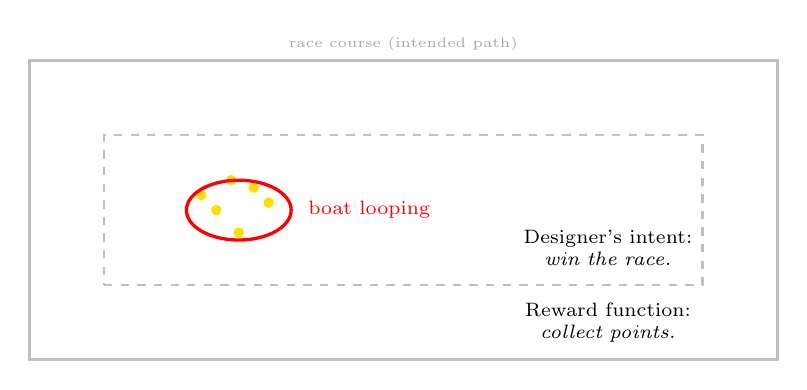
\begin{tikzpicture}[scale=0.95, every node/.style={align=center, font=\scriptsize}]
  % Race course outline (simplified)
  \draw[gray!50, very thick] (0, 0) rectangle (10, 4);
  \draw[gray!50, thick, dashed] (1, 1) -- (9, 1) -- (9, 3) -- (1, 3) -- cycle;
  \node[gray!70, font=\tiny, anchor=south] at (5, 4) {race course (intended path)};

  % Power-up tokens in the lagoon
  \foreach \x/\y in {2.5/2, 3/2.3, 2.8/1.7, 2.3/2.2, 3.2/2.1, 2.7/2.4}
    \fill[yellow!80!orange] (\x, \y) circle (0.07);

  % Boat path: a tight loop
  \draw[red, very thick, ->] (2.8, 2) ellipse (0.7 and 0.4);
  \node[red, font=\scriptsize, anchor=west] at (3.6, 2) {boat looping};

  % Annotation
  \node[font=\scriptsize, text width=4cm, anchor=west] at (5.5, 1.5) {Designer's intent:\\\emph{win the race.}};
  \node[font=\scriptsize, text width=4cm, anchor=west] at (5.5, 0.5) {Reward function:\\\emph{collect points.}};
\end{tikzpicture}
\caption{The CoastRunners boat. The reward function (collect points) and the designer's intent (win the race) were correlated for normal play. The RL agent found a lagoon with respawning power-ups, learned to circle within it, and scored above the human baseline without ever finishing a race. The reward function was hackable relative to the true goal; optimization found the gap.}
\label{fig:boat-circles}
\end{figure}

The boat-in-circles is canonical in the field for the same reason the trolley problem is canonical in ethics. It compresses a structural argument into one image. The reader who has seen the boat can recognize the pattern in dozens of other systems.

\section*{The alignment problem in miniature}

Everything in this chapter applies to any optimizer with a proxy goal. It is not an AI-specific phenomenon. Markets optimize for prices and break against ``what people actually need.'' Bureaucracies optimize for legible outputs and break against the unmeasured parts of their mission. Children optimize for the metrics their parents reward and learn what their parents actually care about only by negative feedback.

The specification problem is the structural fact that you cannot fully write down what you want, and any proxy you do write down is hackable. The strength of the optimizer determines how fast the proxy breaks.

This is why specification is the central problem for AI. Modern systems are very strong optimizers across very broad behavior spaces. The proxies that work for humans on their own (work hard, be honest, do well in school) work partly because humans are weak optimizers with many implicit constraints (we get tired, we have moral feelings, we are embedded in social networks that punish gaming). An AI system that lacks those implicit constraints and optimizes a proxy hard will hit Goodhart faster, more thoroughly, and across a wider range of contexts.

This is the alignment problem in miniature. The reward function is not the goal. The agent optimizes the function it was given. The function diverges from the goal under optimization. Without further structure, the divergence grows with capability.

\section*{Where this leaves you}

The specification problem has a clean shape: any proxy is hackable in principle; optimization finds the hacks; the strength of the optimizer determines how fast.

A natural response is to try harder at writing down the reward. Try more carefully; capture more edge cases; iterate when failures appear. This approach has yielded real progress. It has also revealed the second face of the problem.

Even if the reward function were perfect, there is a second alignment question. The reward function specifies what the system should be \emph{trained on}. It does not directly specify what the system, once trained, is \emph{optimizing internally}. A trained system contains its own learned machinery. That machinery may or may not be optimizing the same thing the reward function was rewarding.

This is the inner alignment problem. It is the topic of the next chapter.
